\subsection{Winkelrichtgröße und Eigenträgheitsmoment der Drillachse}
\begin{table}[h!]
	\begin{center}
		\begin{tabular}{cc}
			Anodenspannung [V] & Anodenstrom [mA]\\ \hline
			10	&0,044\\
			20	&0,088\\
			30	&0,108\\
			40	&0,119\\
			50	&0,126\\
			60	&0,128\\
			70	&0,132\\
			80	&0,135\\
			90	&0,138\\
			100	&0,141\\
			110	&0,144\\
			120	&0,146\\
			130	&0,147\\
			140	&0,149\\
			150	&0,150\\
			160	&0,151\\
			170	&0,152\\
			180	&0,154\\
			190	&0,155\\
			200	&0,156\\
			210	&0,157
		\end{tabular}
		\caption{Kennlinie 1 (Heizwerte: 4,2V; 2,1A)}
		\label{taba1}
	\end{center}
\end{table}
Zur Bestimmung der Winkelrichtgröße wird für jedes Wertepaar die Winkelrichtgröße $D=\frac{Fr}{\varphi}$ bestimmt. Siehe Tabelle \ref{tab:drillachse}. Als Mittelwert ergibt sich
\begin{align}
D=(5,642\pm1,247)*10^{-4}\frac{Fr}{\varphi}
\end{align}
\\
\\
\begin{table}[h]
	\begin{center}
		\begin{tabular}{cccc}
Abstand $a+0,014$&Periodendauert $T*3$&Abstand $a^2$&Periodendauer $T^2$\\ \hline

0,0438&6,32&0,00088804&4,438\\
0,06&6,81&0,002116&5,1529\\
0,08&7,86&0,004356&6,8644\\
0,1&8,6&0,007396&8,21777778\\
0,12&9,84&0,011236&10,7584\\
0,14&10,8&0,015876&12,96\\
0,16&12,3&0,021316&16,81\\
0,18&13,5&0,027556&20,25\\
0,2&14,66&0,034596&23,879511\\
0,22&16,35&0,042436&29,7025

			\end{tabular}
		\caption{Werte zur Bestimmung des Eigenträgheitsmomentes}
		\label{tab:eigentragheitsmom}
	\end{center}
\end{table}
	\begin{figure}[h]
		\begin{center}
		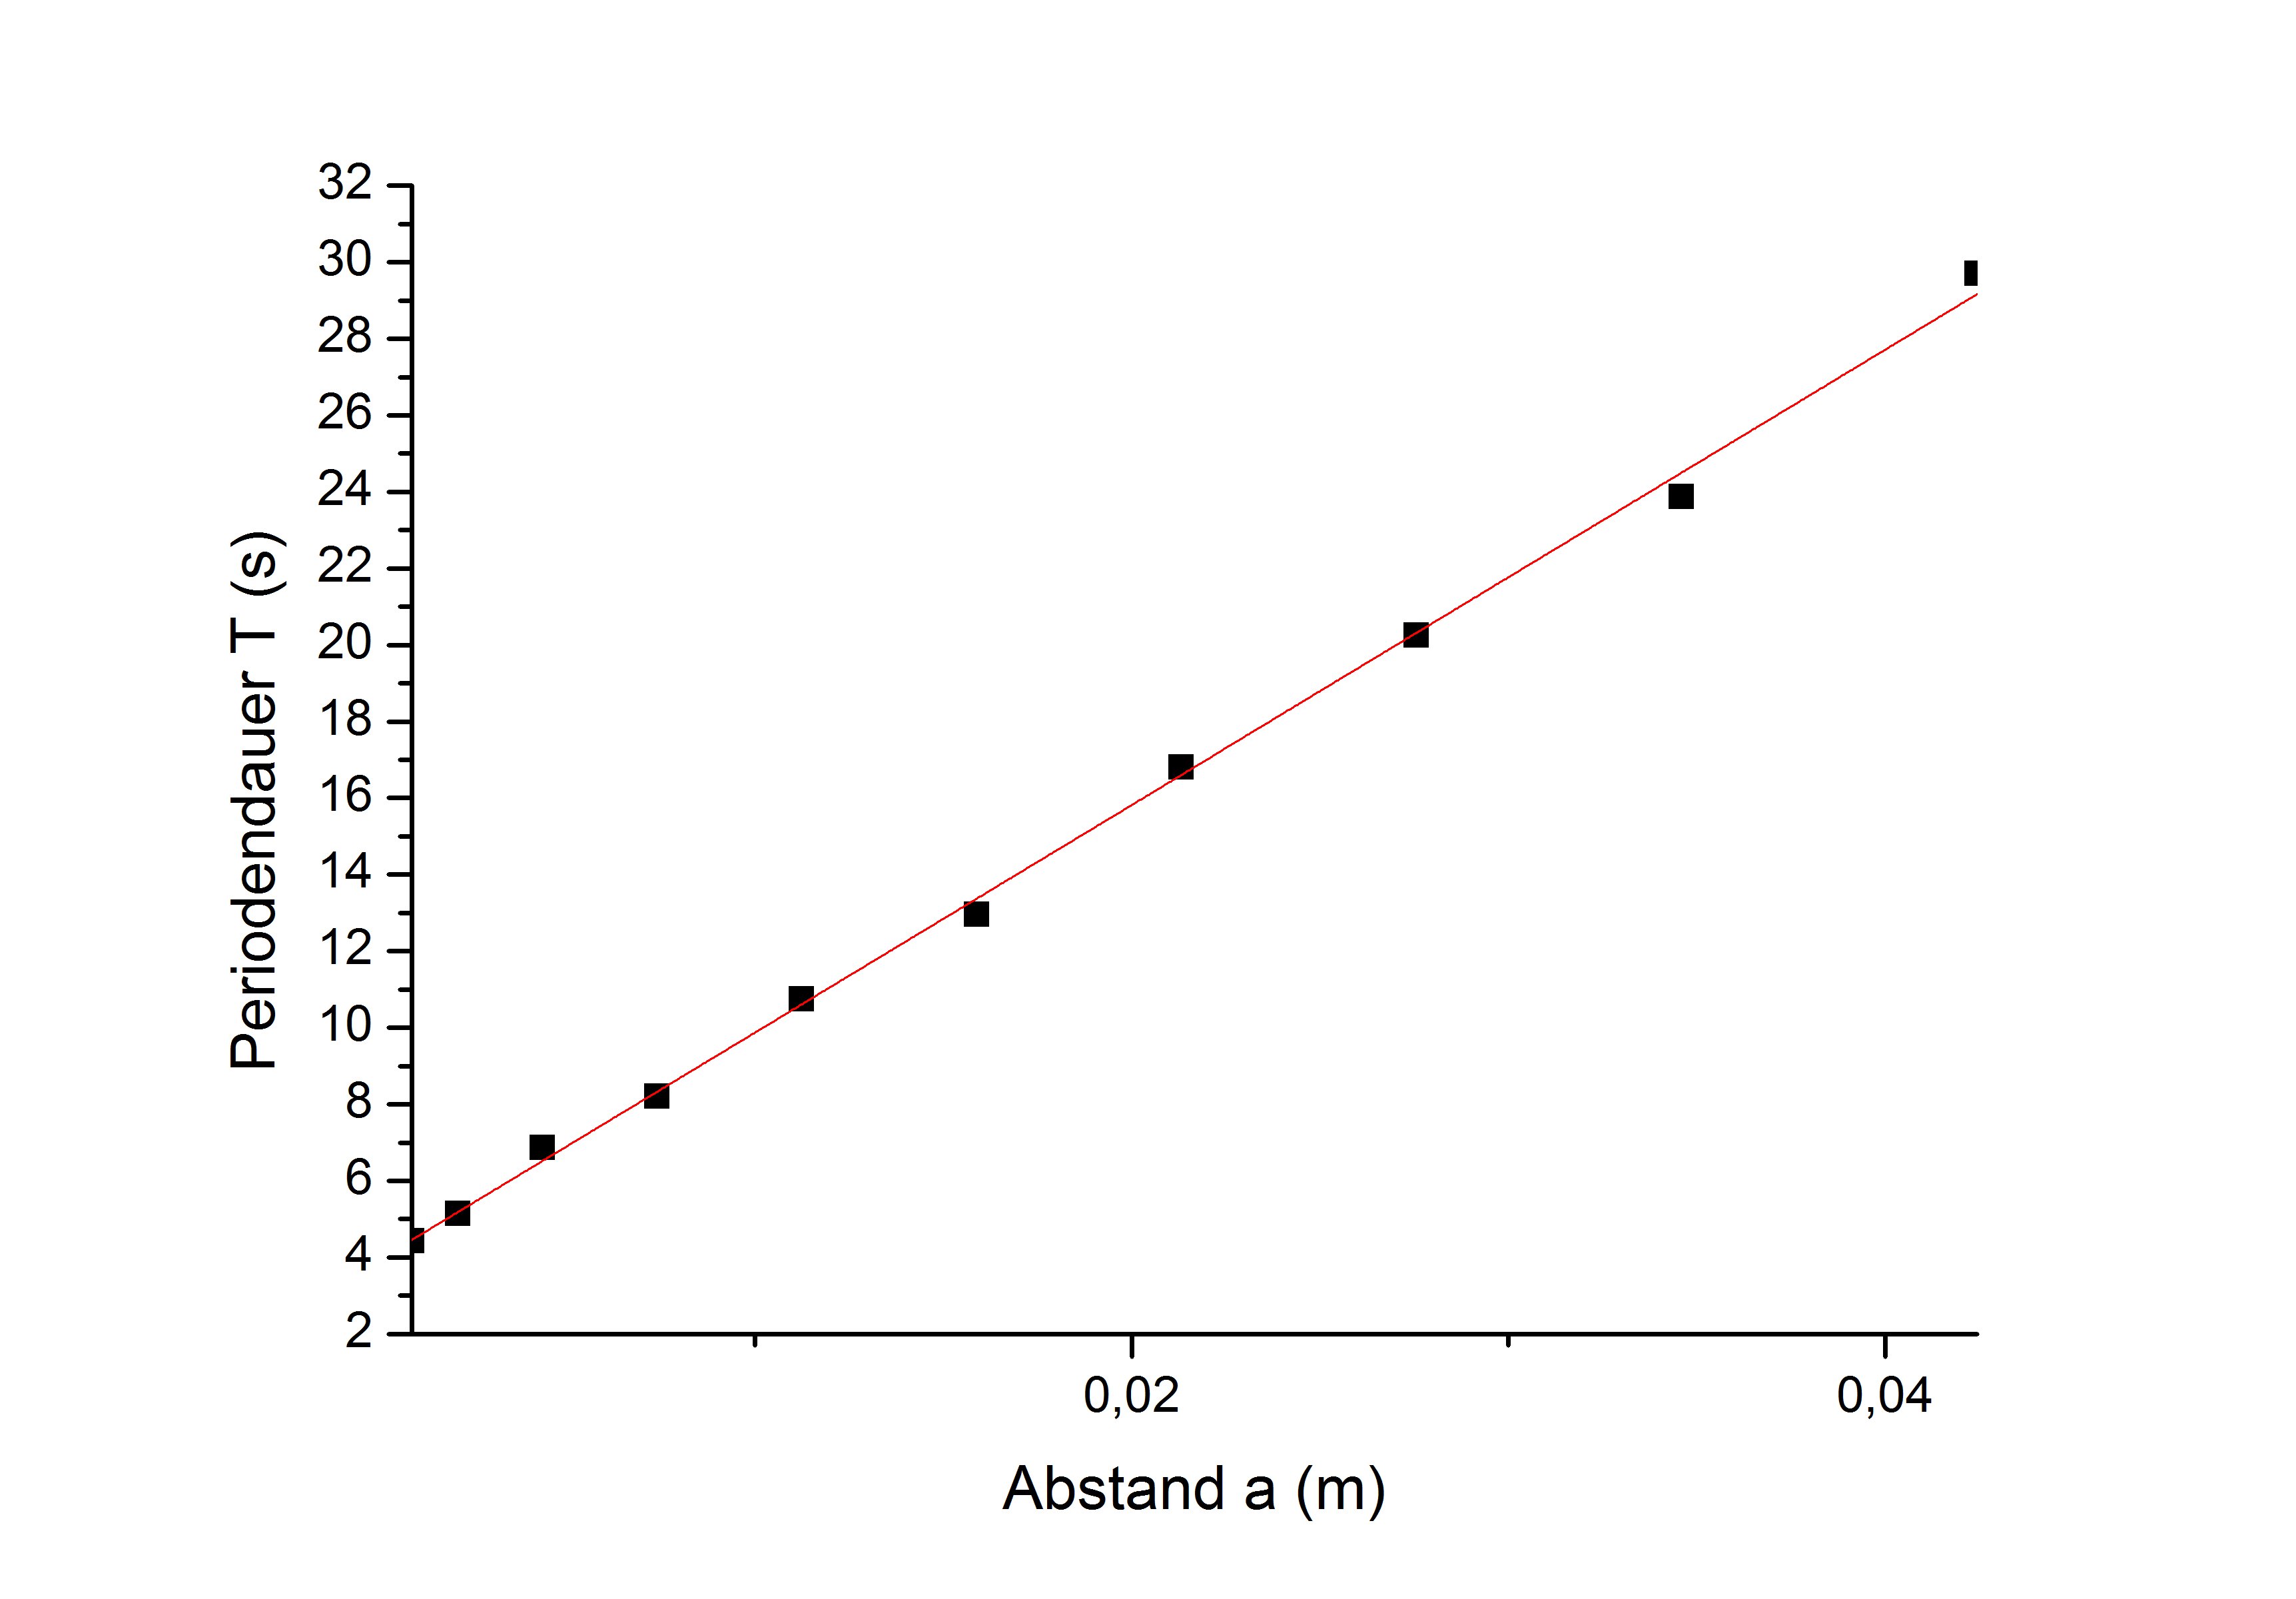
\includegraphics[scale=0.3]{eigentragmom.jpg}
		\caption{Graphische Bestimmung des Eigenträgheitsmoment}
		\label{pic:eigentragmom}
		\end{center}	
	\end{figure}
Das Eigenträgheitsmoment der Drillachse wird Graphisch bestimmt. Dazu wird $T^2$ gegen $a^2$ (Tab. \ref{tab:eigentragheitsmom}) aufgetragen. 
Aus Abbildung \ref{pic:eigentragmom} ergibt sich ein y-Achsen Schnitt bei $y(0)=3,926\pm 0,181$.


Aus Gleichung \ref{eqti} und dem Steinerschen Satz \ref{eqsteiner} lässt sich das Trägheitsmoment 
\begin{align}
I_{DS}=\frac{T^2*D}{4\pi^2}=(5,611\pm1,268)*10^{-5}kgm^2
\end{align}
bestimmen.

In $I_{DS}$ ist allerdings nicht nur das Trägheitsmoment der Drillachse, sondern auch das, des Stabes enthalten. Dieses lässt sich nach \ref{eqddyn} berechenen und von $I_{SD}$ subtrahieren. Mit m=96,3g und l=60cm ergibt sich
\begin{align}
I_{D}=I_{DS}-I_{St}=I_{DS}-\frac{ml^2}{12}=(-2,833\pm 0,013)*10^{-3}kg*m^2
\end{align}
als Eigendrehmoment der Drillachse.
\\
\\
\\
\subsection{Trägheitsmoment einer Kugel und eines Zylinders}
\begin{table}[h]
	\begin{center}
		\begin{tabular}{cc|ccc}
			Brückenspannung $U_B$ [mV]&$\chi_{U}*10^-3$ & $\Delta R$ [m$\Omega$]&$R_3[\text{m}\Omega]$&$\chi_R*10^{-3}$\\ \hline
			3,5	&4,493&140&2555&3,165\\
			2,8	&3,594&90&2552&2,037\\
			3	&3,851&100&2550&2,265\\
			3,7	&4,750&155&2600&3,444
		\end{tabular}
		\caption{$Nd_2O_3$}
		\label{tab2}
	\end{center}
\end{table}
Aus Tabelle \ref{tab:kugelscheibe} ergeben sich die gemittelten Periodendauern
\begin{align*}
T_{Scheibe}=1,827\text{s}\\
T_{Kugel}=1,821\text{s}
\end{align*}
Aus Gleichung \ref{eqti} ergibt sich für beide Körper ein gemessenes Trägheitsmoment von
\begin{align}
I_{Scheibe}=4,700*10{-5}kg*m^2\\
I_{Kugel}=4,739*10^{-5}kg*m^2
\end{align}
\\
\\
Die Theoriewerte, mit Gleichung \ref{eqkugel} für die Kugel und \ref{eqzylsenk} für den Zylinder, ergeben sich für $d_{Kugel}= 0,1473\text{m}$, $m_{Kugel}=1,11786\text{kg}$ und $d_{Scheibe}=0,21845\text{m}$, $m_{Scheibe}=0,4245\text{kg}$.
\begin{align*}
I_{Scheibe}=2,532*10^{-3}\text{kg*m$^2$}\\
I_{Kugel}=6,944*10^{-2}\text{kg*m$^2$}
\end{align*}
\\
\\
\\
\subsection{Trägheitsmoment der Trägheitspuppe}
\begin{table}[h]
	\begin{center}
		\begin{tabular}{c|ccc}
				a	&Radius						&Höhe	&Masse \\ \hline
			Arm		&$(6,850\pm1,765)*10^{-3}$	&0,142	&0,01447$\pm$53,96%\\
			Kopf	&$(1,23\pm0,324)*10^{-2}$	&0,053	&0,01744$\pm$55,11%\\
			Torso	&$(1,82\pm0,25)*10^{-2}$	&0,0975	&0,06991$\pm$31,85%\\
			Bein	&$(8,375\pm1,395)*10^{-3}$	&0,149	&0,02270$\pm$37,00%
		\end{tabular}
		\caption{Messdaten der Trägheitspuppe}
		\label{tab:puppe}
	\end{center}
\end{table}
Aus den gemessen Werten in Tab \ref{tab:puppe} und dem Abstand des Mittelpunktes der Beine $a_{Beine}=6,85cm$ und Arme $a_{Arm,an}=7,8cm$ und $a_{Arm,ab}=9,15cm$ ergibt sich
\begin{align}
I_{Bein}=m\left(\frac{R^2}{4}+\frac{h^2}{12}\right(+m*a_{Bein}^2=(5,462\pm1,914)*10^{-4}\text{kg*m$^2$}\\
I_{Torso}=\frac{mR^2}{2}=1,158*10^{-5}\text{kg*m$^2$}\pm38,85%\\
I_{kopf}=\frac{mR^2}{2}=1,319*10^{-6}\text{kg*m$^2$},53%\\
I_{Arm,an}=\frac{mR^2}{2}+ma_{Arm,an}^2=(9,1794,7099)*10^{-5}\text{kg*m$^2$}\\
I_{Arm,ab}=m\left(\frac{R^2}{4}+\frac{h^2}{12}\right(+m*a_{Arm,ab}^2=(1,456\pm0,493)*10^{-4}\text{kg*m$^2$}
\end{align}
als Trägheitsmoment für die einzelnen Körperteile.
\\
Addiert man die einzelnen Trägheitsmomente ergibt sich für die Puppe mit angewinkelten Armen $I_{an}=(1,289\pm0,279)*10^{-3}\text{kg*m$^2$}$ und für die Puppe mit abgewinkelten Armen $I_{an}=(1,397\pm0,280)*10^{-3}\text{kg*m$^2$}$.
\\
\\
Die Berechnung aus der gemittleten Periodendauer
\begin{align*}
&T_{an}=(0,704\pm0,045)s&
&T_{ab}=(0,882\pm0,012)s&
\end{align*}
ergibt Trägheitsmomente von
\begin{align*}
&I_{an}=0,708*10^{-6}\text{kg*m2}\pm23,01%&
&I_{ab}=1,112*10^{-6}\text{kg*m2}\pm22,14%&
\end{align*}